\chapter{Empirical Studies} \label{sec:empirical-studies}

This chapter presents the empirical studies conducted to investigate and verify the theory and hypothesis laid out in the previous chapter. The objectives of these experiments are to show that deep recurrent neural networks can learn to perform basic arithmetic and that the presence of shared symbols improves the accuracy of these networks when trained using an impoverished dataset. Moreover, we aim to show that the symbolic information presented to the models during training perform the same role that the symbolic knowledge shared between human learners performs. We do this by showing that in the presence of symbols, artificial neural networks are able to discover an algorithm that generalizes to all instances of the problem.

Our experimentations are divided into three groups based on the overall objective of the experiments. The first set of experiments presented in Section \ref{sec:empirical-studies-sequential-models-experiments} aims to prove our hypothesis by comparing the effectiveness of recurrent neural networks trained in the presence of symbols with that of the same networks trained without symbols. The second experimental group described in Section \ref{sec:empirical-studies-explaining-the-role-of-symbols} is meant to explain the role that symbols play in improving a model's accuracy. Finally, Section \ref{sec:empirical-studies-temperature-encoding-experiments} presents  experiments that show how symbols allow the recurrent neural networks to learn an algorithm that captures a general solution to the problem of learning mathematical operations. 

We begin this chapter by providing a general overview of how the experiments are conducted and how the results are compared. Next, we describe the technology and environment on which we developed and executed our experiments. Then we present our experiments, laying out in detail the objective, methodology and results of each experiment. A discussion is provided after each experiment analyzing the results and comparing them to that of previous experiments. In the next and final chapter we provide a summary of the outcomes of our research and how it can be further developed.

\section{Experimental Process and Model Evaluation} \label{sec:empirical-studies-model-evaluation}

This chapter presents seven experiments that investigate the main hypothesis and objectives set out in Chapter 3. The experiments involve training recurrent neural network models, specifically those based on LSTM units to compare the effectiveness of two or more methods of training these networks. The methods are usually variations of training the models in the presence or absence of symbolic features. After the models are trained, they are then tested on independent test datasets to determine each model's accuracy. The accuracy is the percentage of the number of operations a trained neural network is able to successfully complete relative to the entire dataset. Models are compared based on their accuracies and the ones with the highest score are considered most successful at accomplishing their task.

The process of developing the models involves iteratively training the neural networks on a training set. Each iteration is called an epoch and after every epoch a validation dataset is applied to the neural network using the set of weights obtained so far in the training process. An optimum set of weights is always maintained and is replaced with the current set if the current set outperforms the older set on the validation data. Validation is used to prevent overfitting and to also determine when to stop training. The model is trained for a large predetermined number of epochs. However, a stopping condition is applied where, if the network fails to find a better set of weights than the current optimum after a set number of iterations, training is terminated and the current optimum weights are returned as the final trained model. Section \ref{sec:background-artificial-neural-networks} provides more details on training artificial neural networks.

Most experiments gather and present the following four metrics for each neural network model developed:
\begin{itemize}
	\item Mean Accuracy: After each model is fully trained the test set is applied to obtain the model accuracy. The training and testing of each model is repeated five times with a different distribution of training, validation and test data based on k-fold cross-validation where k is set to 5. The mean accuracy is then calculated and this becomes the accuracy score of the model.
	\item Standard Deviation: The standard deviation of the accuracies obtained from each training attempt is calculated. Standard deviation is used to verify the quality of the results by providing a measure of a model's variance. Too much variance can lower the confidence in the results. Standard deviation is used to calculate the remaining two metrics.
	\item Hypothesis Test: The p-value from a standard hypothesis t-test is used to determine the statistical significance of the results. Typically values less than 0.05 means that the null hypothesis is invalid and therefore the results support the theory being tested.
	\item 95\% Confidence Interval: The confidence interval is the statistical margin of error that is considered when comparing two or more results.
	We usually display the mean accuracy, standard deviation and p-value in tables and show the mean accuracy along with the 95\% confidence interval on graphs.
\end{itemize}

\section{Environment} \label{sec:empirical-studies-environment}

Here we describe the hardware and software environments that were used to develop, train and test the neural network models used in the experiments discussed later in this chapter. Typically, the amount of hardware resources needed increases with the size of our datasets\cite{Bengio07scalinglearning}. Since we are deliberately training these neural network models on limited datasets, common off the shelf laptop or desktop computers can be used to replicate these experiments.

All of our models were developed and trained on a laptop with the following specs:
\begin{itemize}
	\item Make and model: Apple MacBook Pro (Early 2015)
	\item CPU: 2.7 GHz Intel Core i5
	\item Memory: 8 GB 1867 MHz DDR 3
	\item Storage: 120 GB Flash Storage
\end{itemize}	
All experiments were validated using k-fold cross-validation where k is set to 5. This means that each experiment was repeated five times. The time it took to run each experiment varied depending on the type of dataset used. The combined average time for all five attempts of the experiments based on images of handwritten digits was around ten hours. The average time for the experiments based exclusively on symbols was about one hour.

With regards to the software technology used:
\begin{itemize}
	\item Python 2.7 is used to code the scripts that construct, train and test the neural network models.
	\item NumPy is a Python library that allows Python's numerical datatypes to represent real numbers with higher precision. It also extends the capabilities of Python's lists to allow for matrix manipulation. TensorFlow and Keras depend on NumPy for their internal workings.
	\item TensorFlow is a native library with a Python wrapper that allows programmers to express mathematical processes like matrix multiplication and gradient descent training in the form of a process graph which Tenserflow can then offload to either a CPU or GPU for execution. Expressing algorithms using process graphs allows the neural network architectures being developed to be abstracted from specific implementations that target CPU or GPU powered machines and therefore enables TensorFlow to optimize the underlying implementation based on the resources available.
	\item Keras is an API that provides neural network developers the ability to specify architectures as well as hyper parameters to TensorFlow without having to manually program these constructs from scratch. This allows researchers to experiment with their theories without worrying about the validity of their implementations.
\end{itemize}	

Alongside the above technologies, the following were also used to format and analyze the results:
\begin{itemize}
	\item Microsoft Excel is used to compile and analyze the results as well as generate the charts presented in the coming sections.
	\item PIL is a Python library that allows developers to generate images. The images included in the sections providing qualitative analysis of our models are generated using PIL.
\end{itemize}

\section{Sequential Models Experiments} \label{sec:empirical-studies-sequential-models-experiments}

In Section \ref{sec:theory-approach-methodology-sequential-models} we explained how basic arithmetic operations, namely addition, subtraction, multiplication and division, can be learned using sequential models such as recurrent neural networks. We also introduced two approaches to providing symbols to neural networks while training; explicit and implicit symbols. This first set of experiments applies this sequential modeling technique to our problem of learning with symbols. We also compare the accuracies of using the two different approaches to providing symbols we discussed earlier, explicit symbols compared to implicit symbols. The overall objective of these experiments is to validate our hypothesis.

\subsection{Experiment 1: Using Symbols to Improve the Effectiveness of Learning} \label{sec:experiment-1}

\subsubsection{Objective}

The goal of this experiment is to demonstrate the validity of our hypothesis by showing that the presence of a clear and concise symbolic representation of the input data improves the learning accuracy of the models developed. The symbols are analogous to the shared knowledge used by human learners to overcome the difficulty in learning from a limited number of noisy examples as discussed in Section \ref{sec:theory-hypothesis}. This first experiment deals with models trained to perform addition only. Later experiments will expand the dataset to include all four basic arithmetic operations.

\subsubsection{Method}

We developed five models based on recurrent neural networks, specifically those based on LSTMs, that learn to sequentially add images of handwritten digits (see Figure \ref{fig:noisy-mnist}). When properly trained the network models can be queried with a sequence of two images, each representing a single digit, followed by an image of the ``+" operator.  The network will output two one-hot vectors representing the estimate of the sum of the input digits. One-hot vectors have all their features set to 0 except for the feature corresponding to the value being represented which is set to 1.

Alongside the handwritten digit input channel, the networks also have a second input channel meant to receive only a standard set of symbols. In the case of numeric digits, the symbols are of the digits zero through nine clearly rendered in a standard font. See Figure \ref{fig:symbols} for the symbolic images used in the experiment. After the five models are trained, the test set is applied to compare the effect of the two approaches of providing symbolic information, mentioned in Section \ref{sec:theory-approach-methodology-sequential-models}, on the accuracies of performing the addition, to the cases of having no symbolic data and only symbolic data.

As discussed in Section \ref{sec:theory-approach-the-mnist-dataset}, the MNIST dataset of handwritten digits is used to train and test all the models developed for all our experiments. A limited subset is sampled from the larger MNIST dataset to create an impoverished collection of examples that are used to train and test our models. The dataset is composed of two single digit inputs followed by the operator. For each of the 100 two digit combinations, we randomly sample ten examples from the MNIST database. For example, the 0 + 0 combination has 10 different examples sampled, the 0 + 1 combination has another 10 examples and so on. This number was chosen because it impoverishes the dataset and also provides room for improvement when introducing symbols. In total, one thousand different input/output pairs are composed. Figure \ref{fig:dataset-examples} shows example combinations, each combination having one sample from the MNIST dataset. Constructing the dataset in that way ensures that there is sufficient balance of training and testing examples for each combination.

\begin{figure}[t]
	\centering
	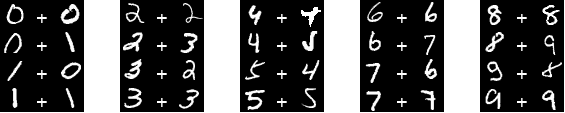
\includegraphics[max width=\textwidth]{dataset-examples}
	\caption{Some of the combinations of operands used for the experiment. Each combination shows only one sample selected from the MNIST dataset.}
	\label{fig:dataset-examples}
\end{figure}

A 5-fold cross-validation (discussed in Section \ref{sec:background-artificial-neural-networks-feed-forward-neural-networks}) approach is used to break down the dataset into a training, validation and test set such that for each combination of digits, six samples are used for training, two samples for validation and another two for testing. Since $k$ is set to 5, the training and testing of each of the five models is repeated five times, where the training, validation and testing samples for each combination are shuffled. The models for this experiment are exposed to all possible combinations of single digit operands during training. Some of the later experiments will only use a subset of the combinations for training and the rest for testing. After repeating the experiment five times for each model and recording the accuracies obtained from testing with the test sets, the mean accuracy and standard deviation for each model are calculated and used to compare the experiments graphically. A Hypothesis t-Test is also used to check the statistical difference of the means.

All networks trained have the same architecture, varying only in terms of the number of inputs. The architecture consists of two hidden LSTM layers, 512 units each, fully connected to an output layer, 20 units in length, composed of two one-hot vectors. This architecture was the result of trial and error and was found to have sufficient representation for the most difficult task at no detriment to the other tasks. The networks are trained using the Adam optimizer with the mean square error as the loss function and a learning rate of 0.001. Training is performed over 200 epochs (found to be sufficient for all methods) in batches of 100 and the set of weights performing best on the validation set is saved.  When evaluating the models, only noisy handwritten images are input and no symbol images are provided. The following paragraphs describe the five different architectures and training sets used.

\begin{figure}[t]
	\centering
	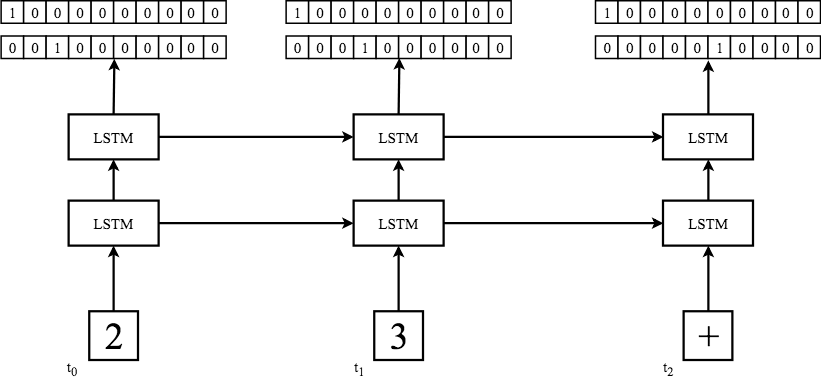
\includegraphics[max width=\textwidth]{sequential-model-symbols-only}
	\caption{Symbols Only (SO). A deep LSTM network that accepts a sequence of two operands and an operator. The operands are provided as the consistent symbol digits.}
	\label{fig:sequential-model-symbols-only}
\end{figure}

\paragraph{Symbols Only (SO).} The model learns to perform classification and addition using only the standard symbols (see Figure \ref{fig:sequential-model-symbols-only}). The input is a sequence of three 28x28 images, that are fed to the network one after the other. The first two images are that of the digits rendered clearly using a standard font. The third image is the plus operator. At each of the first two time steps the model is trained to classify the incoming digits producing two one-hot vectors representing the least and most significant digits of the input. Typically, the most significant digit will always be zero on these two time steps since we only use single digit inputs. When the plus sign is provided on the third time step, the network performs the addition operation, producing the result at the two one-hot vectors. The goal of training this model is to show that it is quite easy to do so using clear and consistent symbols.

\begin{figure}[t]
	\centering
	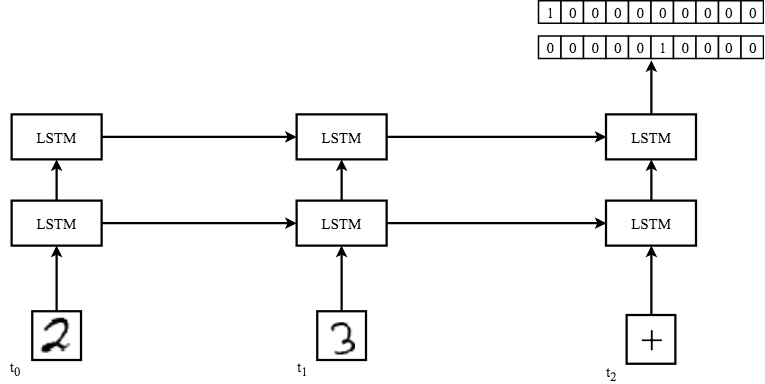
\includegraphics[max width=\textwidth]{sequential-model-noisy-only}
	\caption{Noisy Inputs Only (NO). A deep LSTM network that accepts a sequence of two operands and an operator. Only noisy operands are provided.}
	\label{fig:sequential-model-noisy-only}
\end{figure}

\paragraph{Noisy Inputs Only (NO).} The model learns to perform the addition using noisy handwritten digits without having to output the proper classes in the intermediate stages of the recurrent network (see Figure \ref{fig:sequential-model-noisy-only}). The input is a sequence of three 28x28 images, that are fed to the network one after the other. The first two images are that of noisy handwritten digit operands. The third image is the plus operator rendered in a standard font.  The goal of training the model using this method is to investigate the effectiveness of a network that is trained without the presence of symbols.

\begin{figure}[t]
	\centering
	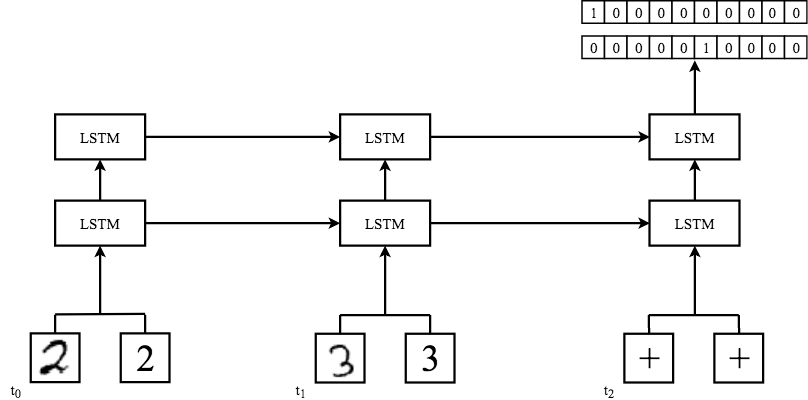
\includegraphics[max width=\textwidth]{sequential-model-symbols-noisy}
	\caption{Noisy and Symbol Inputs (NS). A deep LSTM network that accepts a sequence of two operands and an operator. Both the noisy operands and their corresponding symbolic information are provided alongside one another.}
	\label{fig:sequential-model-symbols-noisy}
\end{figure}

\paragraph{Noisy and Symbol Inputs (NS).} This model learns to perform addition without having to output the proper classes in the intermediate stages of the recurrent network (see Figure \ref{fig:sequential-model-symbols-noisy}). The input is a sequence of three pairs of 28x28 images, that are fed to the network one after the other. The first pair of images are of the first noisy handwritten digit operand and its matching standard symbolic digit. The second pair of images are for the second digit operand. The third pair of images are both the standard plus operator. The goal is to investigate the effect of introducing the clear symbol channel as an input (the explicit symbol) on the accuracy of the network.

\begin{figure}[t]
	\centering
	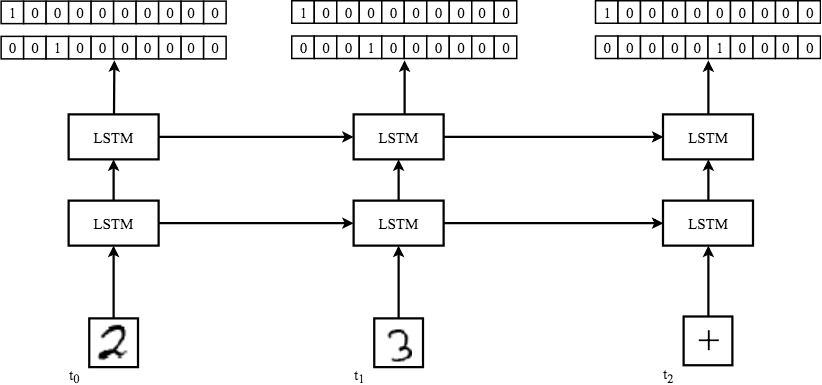
\includegraphics[max width=\textwidth]{sequential-model-noisy-classification}
	\caption{Noisy Inputs Only with Intermediate Classification (NC). A deep LSTM network that accepts a sequence of two operands and an operator. Noisy digits are provided as inputs and the network is trained to output the classes of each digit before performing the operation.}
	\label{fig:sequential-model-noisy-classification}
\end{figure}

\paragraph{Noisy Inputs Only with Intermediate Classification (NC).} The model learns to perform classification and addition on noisy digits only(see Figure \ref{fig:sequential-model-noisy-classification}). The input is a sequence of three 28x28 images, that are fed to the network one after the other. The first two images are that of handwritten digit operands. The third image is the plus operator. The model is trained to classify each incoming digit on each of the first two time steps by providing the class (as a one-hot vector) on the output during training and then perform the operation on the third time step. The goal is to investigate the effect of symbols on the accuracy of the network. However instead of using explicit symbols as inputs, the symbol is embedded in the LSTM context. By providing the classes of the handwritten digits while training, we believe that the network learns the symbolic information implicitly in the recurrent weights and then uses this information to aid in performing the mathematical operation.

\begin{figure}[t]
	\centering
	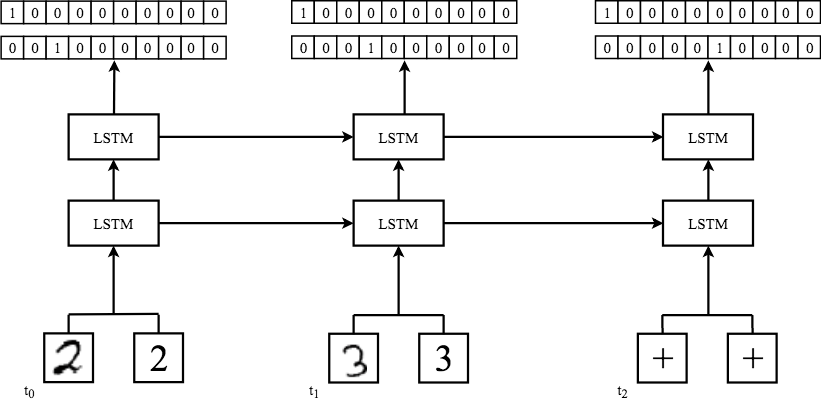
\includegraphics[max width=\textwidth]{sequential-model-noisy-symbol-classification}
	\caption{Noisy and Symbol Inputs with Intermediate Classification (NX). A deep LSTM network that accepts a sequence of two operands and an operator. Both the explicit and implicit symbols are provided.}
	\label{fig:sequential-model-noisy-symbol-classification}
\end{figure}

\paragraph{Noisy and Symbol Inputs with Intermediate Classification (NX).} This last model combines both methods of training used in NS and NC where the input includes the clear symbolic channel and the input classes are also provided on the output channel during training (see Figure \ref{fig:sequential-model-noisy-symbol-classification}). Here we investigate if a combination of the two methods of symbolic input improves on the individual approaches of the previous two methods.

\bigskip

While testing the trained Symbols Only (SO) model, we also test how well that model performs when tested on noisy handwritten digit inputs. We call this testing attempt \textbf{Symbols Tested with Noisy Inputs (SN)}. The objective is to see if training a recurrent neural network using only the idealized symbols will help the resulting model filter out the noise seen in the handwritten digits.

\subsubsection{Results}

\begin{table}[p!]
	\center
	\caption{A comparison of the mean accuracy and standard deviation of the models developed by the five methods. Also shown is the p-value of a hypothesis t-Test when compared to the NO method.}
	\label{tab:experiment-1-results-table}
	\begin{tabular}{ |c|c|c|c| } 
		\hline
		Method & Accuracy (\%) & Standard Deviation  & p-value, t-Test with NO Method\\ 
		SO & 100 & 0 & NA\\ 
		SN & 32.73 & 6.9 & NA\\
		NO & 60.16 & 4.5 & NA \\ 
		NS & 82.63 & 3.7 & 0.00317\\ 
		NC & 84.20 & 2.1 & 0.00102\\ 
		NX & 85.20 & 2.7 & 0.00043\\ 
		\hline
	\end{tabular}
\end{table}

\begin{figure}[p!]
	\centering
	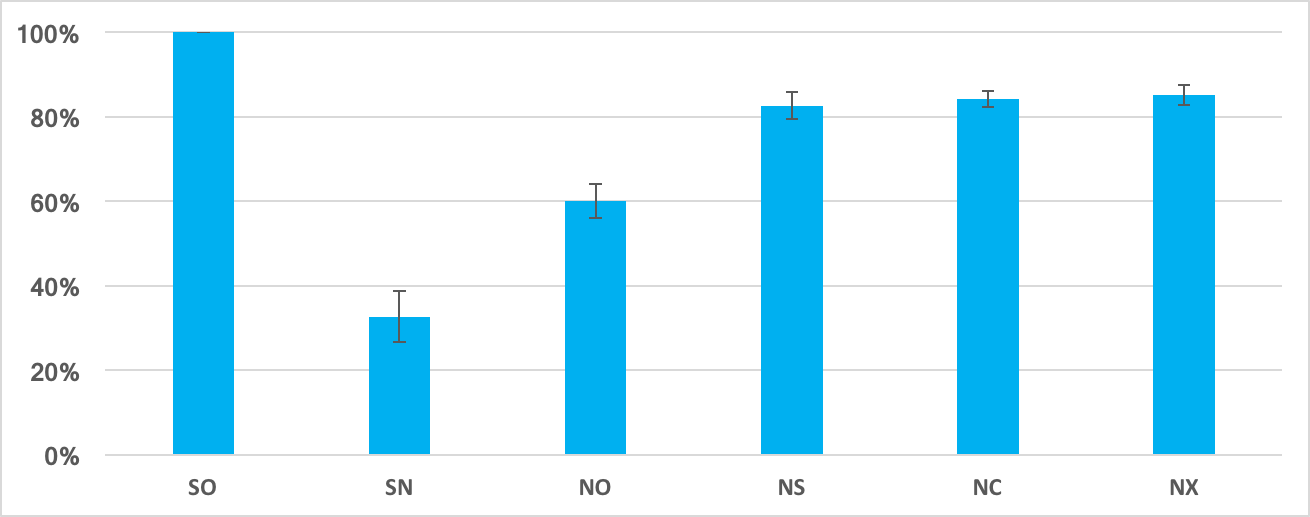
\includegraphics[max width=\textwidth]{experiment-1-results-chart}
	\caption{A comparison of the mean accuracy and 95\% confidence intervals of the models developed by the five methods.}
	\label{fig:experiment-1-results-chart}
\end{figure}

Table \ref{tab:experiment-1-results-table} and Figure \ref{fig:experiment-1-results-chart} compare the scores obtained from evaluating the models after training using the five methods. Training with symbols only (SO) produces the best model given the clear and consistent symbolic images. Training with the noisy handwritten digits only (NO) produces the worst model given the limited number of examples in the dataset. The three methods (NS, NC, NX) that developed models using noisy handwritten images as well as symbolic information show significant improvement over noisy only training. The results also show that there are no significant differences between the two methods of supplying symbols to the networks. However, the models that were trained using intermediate classification (NC and NX) have a smaller standard deviation.

\subsubsection{Discussion}

The experiments show that training a model with symbols results in a significant increase in the network accuracy over the models trained without the presence of symbols. The NC method that developed models to classify the operands as well as compute the addition did particularly well without the need for any additional inputs. The model does not accept a symbolic channel. Instead, by providing proper classification of the input operands while training, the model can be said to develop an implicit symbolic representation of the operands in the LSTM's recurrent context and transfer them from one step to the next.

The results presented in Table \ref{tab:experiment-1-results-table} and Figure \ref{fig:experiment-1-results-chart} show that there is no significant difference in the accuracy of the models trained using implicit symbols (NC) over the models trained with explicit symbols (NS). However, the experiment shows that the implicit symbol (NC) technique provides symbols to the network with the lowest predictive variance and therefore, we will use the implicit symbol technique in subsequent experiments.

Table \ref{tab:experiment-1-results-table} and Figure \ref{fig:experiment-1-results-chart} also show the results of testing the symbols only model (SO) using noisy data (SN). It is clear from the results that the network performs poorly. The model is not able to correctly map from the noisy handwritten digits to the classification labels and therefore is not able to successfully perform the addition.

\subsection{Experiment 2: Expanding Experiment 1 to use all four arithmetic operations} \label{sec:experiment-2}

\subsubsection{Objective}

The goal of this experiment is similar to Experiment 1 where we attempted to verify that the presence of symbols while training an artificial neural network results in significant increases in the network accuracy. Experiment 1 used only the addition operation. This experiment expands the dataset used to include all four arithmetic operations.

\subsubsection{Method}

For this experiment we use the \textbf{Noisy Inputs with Intermediate Classification (NC)} from the previous experiment as the model that is trained in the presence of symbols. Figure \ref{fig:sequential-model-symbols-noisy-times} depicts the NC model learning to do multiplication. \textbf{The Noisy Inputs Only (NO)} model is also used for comparison as the model trained without symbols. NO is slightly modified to provide output on its intermediate time steps. The output provided during training for these intermediate time steps is a vector with all its features set to a dummy value of 0.5 to signify that no symbol is provided. Figure \ref{fig:sequential-model-noisy-only-divide} shows an example of the NO model performing division.

The dataset used for Experiment 1 is expanded to include four different arithmetic operations (addition, subtraction, multiplication and division). For each operation, single digit inputs from the range of 0 to 9 are used to form combinations of operands and for each combination, ten MNIST examples are sampled. For both addition and multiplication, all 100 combinations are included in the dataset. However, for subtraction and division the combinations are selected so that for subtraction, no combinations that would result in negative outputs would be included and for division, division by zero is avoided. K-fold cross-validation is used, with k set to 5, to split the samples of each combination into a training, validation and test set. The training and testing of each model is repeated five times and the accuracy obtained on the test set is recorded for each attempt. Just like in Experiment 1, all combinations of digits are provided for training.

\begin{figure}[t]
	\centering
	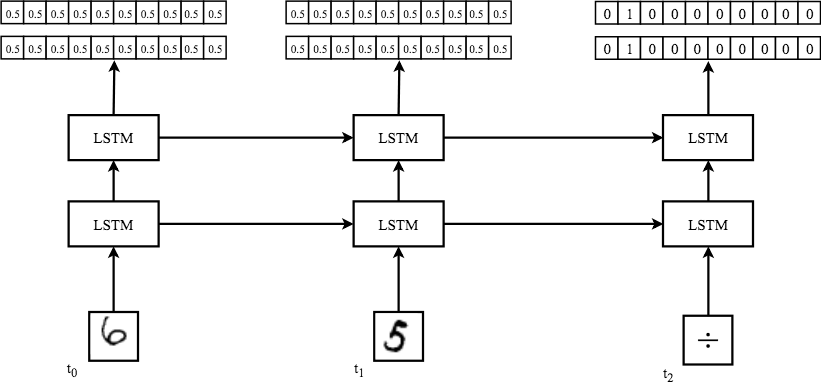
\includegraphics[max width=\textwidth]{sequential-model-noisy-only-divide}
	\caption{The Noisy Inputs Only (NO). A deep LSTM network that accepts a sequence of two operands and an operator modeling the operation: 6 / 5. Only noisy operands are provided. The output represents the quotient and the remainder, which are both 1.}
	\label{fig:sequential-model-noisy-only-divide}
\end{figure}

Both models have the same architectures used in Experiment 1. The models accept a sequence of three 28x28 images. The first two images are of the handwritten digits representing the operands of the operation. The third image is that of the operator. The models output two one-hot vectors representing the least and most significant values of the output at each time step. When each of the operands is presented, the network attempts to output the correct signals on the one-hot vector outputs representing the value of the digit presented on the input. When finally the operator is presented, the network is trained to perform the operation and output the result. Both models use two hidden LSTM layers each with 512 units.

\begin{figure}[t]
	\centering
	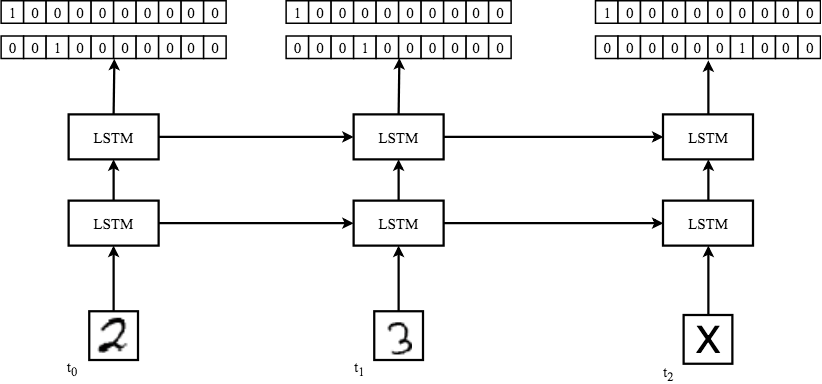
\includegraphics[max width=\textwidth]{sequential-model-symbols-noisy-times}
	\caption{Noisy Inputs with Intermediate Classification (NC). A deep LSTM network that accepts a sequence of two operands and an operator modeling the operation 2 x 3. Both the noisy operands and their corresponding symbolic information are provided alongside one another.}
	\label{fig:sequential-model-symbols-noisy-times}
\end{figure}

\subsubsection{Results}

\begin{table}[p]
	\center
	\caption{A comparison of the mean accuracy and standard deviation of the models trained with and without classification on all four arithmetic operations. Also shown is the p-value of a hypothesis t-Test when compared to the NO method.}
	\label{tab:experiment-2-results-table}
	\begin{tabular}{ |c|c|c|c| } 
		\hline
		Method & Accuracy (\%) & Standard Deviation  & p-value, t-Test with NO Method\\ 
		NO & 60.75 & 0.02 & NA \\  
		NC & 77.36 & 0.03 & 0.00092\\  
		\hline
	\end{tabular}
\end{table}

\begin{figure}[p]
	\centering
	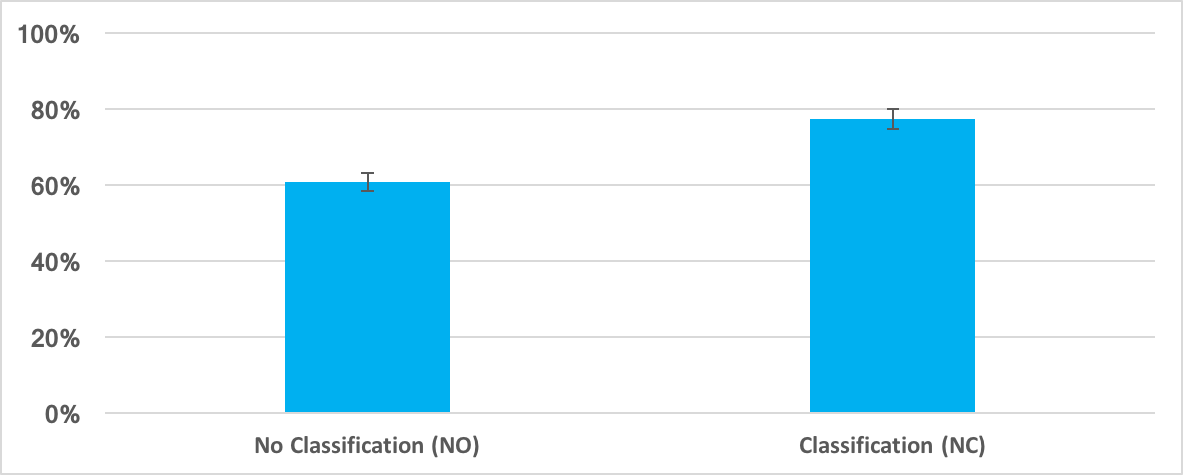
\includegraphics[max width=\textwidth]{experiment-2-results-chart}
	\caption{A comparison of the mean accuracy and 95\% confidence intervals of the models trained with and without classification on all four arithmetic operations.}
	\label{fig:experiment-2-results-chart}
\end{figure}

\begin{table}
	\center
	\caption{The mean accuracies of each arithmetic operation when tested on both the NO and NC models.}
	\label{tab:experiment-2-operations-table}
	\begin{tabular}{ |c|c|c|c|c| } 
		\hline
		Method & Addition (\%) & Subtraction (\%)  & Multiplication (\%) & Division (\%)\\ 
		NO & 63.35 & 60.77 & 61.4 & 57.48\\  
		NC & 78.5 & 77.71 & 80.23 & 73.0\\  
		\hline
	\end{tabular}
\end{table}

\begin{figure}[t]
	\centering
	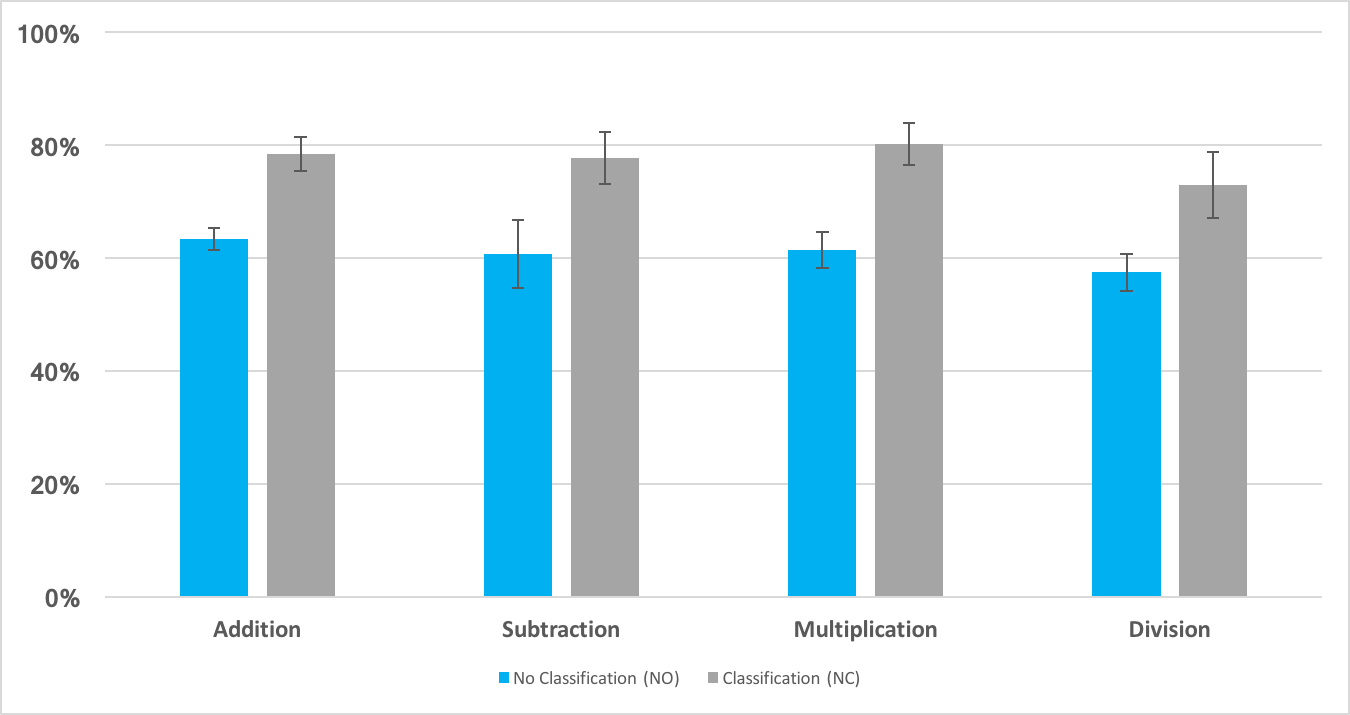
\includegraphics[max width=\textwidth]{experiment-2-operations-chart}
	\caption{A comparison of the mean accuracy and 95\% confidence intervals of each arithmetic operation on both models trained with and without classification.}
	\label{fig:experiment-2-operations-chart}
\end{figure}

Table \ref{tab:experiment-2-results-table} and Figure \ref{fig:experiment-2-results-chart} compare the results of the model trained without symbols (NO) with the model trained with symbols (NC). The model trained in the presence of symbols performs significantly better than the one trained without symbols. Table \ref{tab:experiment-2-operations-table} and Figure \ref{fig:experiment-2-operations-chart} show the accuracies obtained using each of these models when tested on each arithmetic operator independently.

\subsubsection{Discussion}

This experiment shows that the LSTM recurrent neural networks are capable of learning various types of arithmetic operations on images of handwritten digits and that the presence of symbolic knowledge during training significantly improves the accuracy of these models. With the exception of division, Table \ref{tab:experiment-2-operations-table} and Figure \ref{fig:experiment-2-operations-chart} show that when analyzing the accuracies of the models on each operator independently, we see that the mean accuracies are close to one another and close to the overall mean accuracy of the models. Division is a more complicated operation that involves finding a quotient and a remainder which could account of the reduced performance.

\subsection{Experiment 3: Comparing the Effect of Varying the Presence of Symbols on the Accuracy of Training} \label{sec:experiment-3}

\subsubsection{Objective}

In the previous experiments, we showed that the presence of symbols improves the effectiveness of recurrent neural networks in learning to perform arithmetic on images of handwritten digits when training using an impoverished dataset. In Section \ref{sec:theory-hypothesis-multi-task-learning} we proposed that this would be the expected behavior due to the beneficial effect of multi-task learning on all tasks being learned by the recurrent networks. In this experiment we attempt to further demonstrate this benefit.
 
Our goal is to show the relationship between the accuracy of the model in classifying the inputs on the intermediate time steps and the accuracy of the same model in producing the correct output for the given mathematical operation. The existence of this relationship should indicate that by correctly classifying the digits, the recurrent neural network is able to create internal features on the first two time steps that are then used on the third time step to perform the arithmetic operation. In the absence of these clear features, the network would rely only on the noisy handwritten inputs.

Besides establishing the relationship between the classification accuracy and the mathematical accuracy of our models, we also to vary the percentage of symbols included with each training example. The expected outcome here is that the higher the percentage of symbols present, the more accurate the classification accuracy will be and in turn the higher the accuracy of performing the arithmetic operation.

\subsubsection{Method}

The architectures constructed for this experiment are the same as the ones used in the previous two experiments. The models accept a sequence of three 28x28 images. The first two images are of the handwritten digits representing the operands of the operation. The third image is that of the operator. The networks output two one-hot vectors. When each of the operands are presented, the model attempts to output a one-hot encoded vector of the value of the operand. When the operator is presented, the network learns to compute and present the output. Two hidden layers are used each containing 512 LSTM units. All four arithmetic operations are used together during training.

The dataset used in Experiment 2 in Section \ref{sec:experiment-2} is replicated into five sets, with some modifications, for use in this experiment. Each combination now includes eight MNIST samples instead of ten, where four are used for training, two for validation and two for testing. This makes the process of varying symbols easier. Each of the five replicas are modified to vary the number of symbols included with each digit combination during training. The first set has no symbols, meaning a vector with all features set to 0.5 is provided as a dummy output for the intermediate classification time steps. The second dataset has 25\% of the MNIST samples in each combination include a symbol whereas the rest use the 0.5 dummy values. The 25\% symbols are distributed such that, out of the four training samples, one has a symbol and the rest do not. The third dataset has 50\% symbols meaning that out of the four training examples per combination two include their corresponding symbols. The fourth dataset has 75\% of the training examples include symbols, meaning three out of four examples per combination include their corresponding symbol. Finally, the fifth dataset, the 100\% symbols dataset, includes symbols for all examples.

Five models were trained each using one of the datasets described above. The networks were trained using the Adam optimizer with the mean square error as the loss function and a learning rate of 0.001. Training is performed over 200 epochs in batches of 100 and the model performing best on the validation set is saved. Each model is trained five times using 5-fold cross-validation where all digit combinations are used. Instead of recording the accuracy of each model as was done in the previous experiments, here we split the accuracy into four new metrics. They are as follows:
\begin{itemize}
	\item False Classification/False Operation \textbf{(FC/FO)}: The percentage of test samples that classify incorrectly during the intermediate time steps that also produce incorrect outputs for the mathematical operation.
	\item False Classification/True Operation \textbf{(FC/TO)}: The percentage of test samples that classify incorrectly during the intermediate time steps that produce correct outputs for the operation.
	\item True Classification/False Operation \textbf{(TC/FO)}: The percentage of test samples that classify correctly during the intermediate time steps that produce incorrect outputs for the operation.
	\item True Classification/True Operation \textbf{(TC/TO)}: The percentage of test samples that classify correctly during the intermediate time steps that also produce correct outputs for the operation.
\end{itemize}

The epoch number that results in the most optimum set of weights for each percentage of symbols used is also recorded, to understand the effect of symbols on the efficiency of training with and without symbols.

\subsubsection{Results}

\begin{table}[p]
	\center
	\caption{A comparison of the mean FC/FO percentage, standard deviation and the p-value of a hypothesis t-Test when compared to the 0\% symbols model.}
	\label{tab:experiment-3-results-table-fcfo}
	\begin{tabular}{ |c|c|c|c| } 
		\hline
		\% Symbols Present & FC/FO (\%) & Standard Deviation  & p-value\\ 
		0\% & 55.8 & 0.063 & NA \\  
		25\% & 39.80 & 0.03 & 0.00493\\  
		50\% & 26.20 & 0.042 & 0.00141 \\  
		75\% & 17.05 & 0.023 & 0.00033\\  
		100\% & 13.60 & 0.012 & 0.00016\\  
		\hline
	\end{tabular}
\end{table}

\begin{table}[p]
	\center
	\caption{A comparison of the mean FC/TO percentage, standard deviation and the p-value of a hypothesis t-Test when compared to the 0\% symbols model.}
	\label{tab:experiment-3-results-table-fcto}
	\begin{tabular}{ |c|c|c|c| } 
		\hline
		\% Symbols Present & FC/TO (\%) & Standard Deviation  & p-value\\ 
		0\% & 37.55 & 0.0672 & NA \\  
		25\% & 27.95 & 0.0387 & 0.0031\\  
		50\% & 11.50 & 0.0351 & 0.00141 \\  
		75\% & 5.40 & 0.0137 & 0.00084\\  
		100\% & 2.45 & 0.0042 & 0.00016\\  
		\hline
	\end{tabular}
\end{table}

\begin{table}[p]
	\center
	\caption{A comparison of the mean TC/FO percentage, standard deviation and the p-value of a hypothesis t-Test when compared to the 0\% symbols model.}
	\label{tab:experiment-3-results-table-tcfo}
	\begin{tabular}{ |c|c|c|c| } 
		\hline
		\% Symbols Present & TC/FO (\%) & Standard Deviation  & p-value\\ 
		0\% & 3.70 & 0.0106 & NA \\  
		25\% & 15.05 & 0.0214 & 0.00183\\  
		50\% & 23.20 & 0.01024 & 0.02209 \\  
		75\% & 13.55 & 0.0107 & 0.00013\\  
		100\% & 8.15 & 0.0158 & 0.01742\\  
		\hline
	\end{tabular}
\end{table}

\begin{table}[p]
	\center
	\caption{A comparison of the mean TC/TO percentage, standard deviation and the p-value of a hypothesis t-Test when compared to the 0\% symbols model.}
	\label{tab:experiment-3-results-table-tcto}
	\begin{tabular}{ |c|c|c|c| } 
		\hline
		\% Symbols Present & TC/TO (\%) & Standard Deviation  & p-value\\ 
		0\% & 2.95 & 0.0166 & NA \\  
		25\% & 17.20 & 0.0148 & 0.00043\\  
		50\% & 39.10 & 0.0853 & 0.00179 \\  
		75\% & 64.00 & 0.0301 & 0.0\\  
		100\% & 75.80 & 0.0213 & 0.0\\  
		\hline
	\end{tabular}
\end{table}

\begin{figure}[p]%
	\centering
	\subfloat[False Classification/False Operation]{{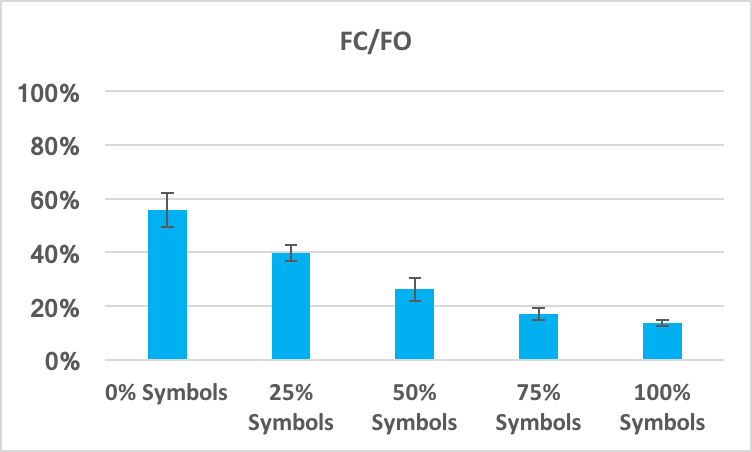
\includegraphics[width=0.5\textwidth]{experiment-3-results-chart-fc-fo} }}\label{fig:experiment-3-results-chart-fc-fo}%
	\subfloat[False Classification/True Operation]{{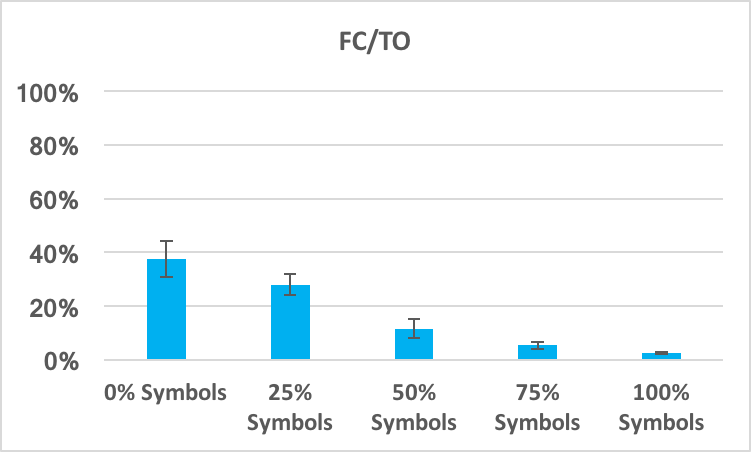
\includegraphics[width=0.5\textwidth]{experiment-3-results-chart-fc-to} }}\label{fig:experiment-3-results-chart-fc-to}%
	
	\subfloat[True Classification/False Operation]{{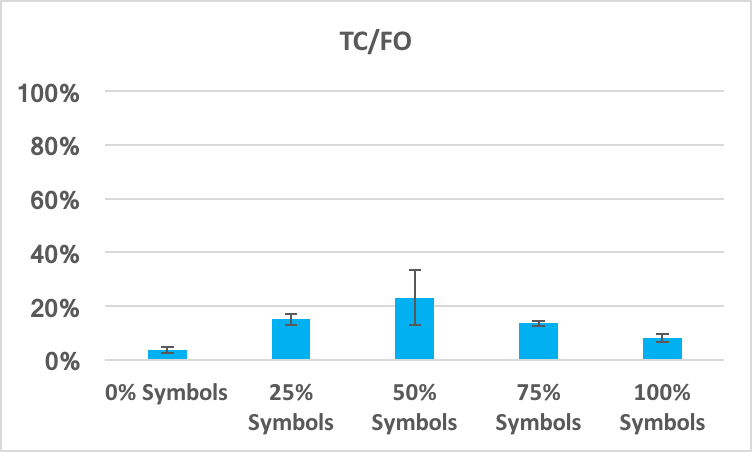
\includegraphics[width=0.5\textwidth]{experiment-3-results-chart-tc-fo} }}\label{fig:experiment-3-results-chart-tc-fo}%
	\subfloat[True Classification/True Operation]{{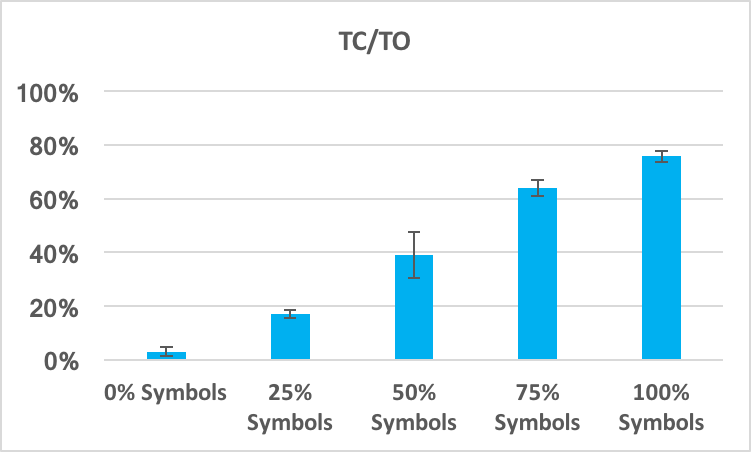
\includegraphics[width=0.5\textwidth]{experiment-3-results-chart-tc-to} }}\label{fig:experiment-3-results-chart-tc-to}%
	\caption{A comparison of the four metrics FC/FO, FC/TO, TC/FO, TC/TO along with their corresponding 95\% confidence intervals for each of the five models developed.}%
	\label{fig:experiment-3-results-chart}%
\end{figure}

Tables \ref{tab:experiment-3-results-table-fcfo} to \ref{tab:experiment-3-results-table-tcto} present the mean FC/FO, FC/TO, TC/FO, TC/TO accuracies for each of the datasets used along with the standard deviations and the p-test score of a hypothesis t-Test compared to the 0\% model. Figure \ref{fig:experiment-3-results-chart} shows the same results presented in graphical form. Table \ref{tab:experiment-3-results-epochs} presents the number of epochs needed for the network to discover the optimum set of weights for each of the five datasets.

\begin{table}[h]
	\center
	\caption{A comparison of the average epoch number at which the optimum weights were discovered for each of the models trained.}
	\label{tab:experiment-3-results-epochs}
	\begin{tabular}{ |c|c| } 
		\hline
		\% Symbols Present & Mean Epoch Number\\ 
		0\% Symbols & 4.2\\  
		25\% Symbols & 10.0\\  
		50\% Symbols & 11.0\\  
		75\% Symbols & 15.8\\  
		100\% Symbols & 38.0\\  
		\hline
	\end{tabular}
\end{table}

\subsubsection{Discussion}

It is clear from Table \ref{tab:experiment-3-results-table-tcto} and Figure \ref{fig:experiment-3-results-chart}(d) that more training examples with symbolic classification data improves the correct output of the operations (TO), particularly when the classification is also correct (TC) (75.8\% of the time with 100\% symbols), and rarely, as shown in Table \ref{tab:experiment-3-results-table-fcto} and Figure \ref{fig:experiment-3-results-chart}(b) when the classification is incorrect (FC) (only 2.45\% of the time with 100\% symbols).

Inversely, as shown in Table \ref{tab:experiment-3-results-table-fcfo} and Figure \ref{fig:experiment-3-results-chart}(a), incorrect output (FO) for a mathematical operator occurs frequently with false classification (FC) (13.6\% of the time with 100\% symbols). It also makes sense that as the percentage of false classifications (FC) declines (due to more symbols in the training set) the percentage of false operation (FO) outputs also declines, because the probability of an operation being performed on the wrong operands decreases.

These results show that the presence of symbols improves the accuracy of classification which in turn improves the accuracy of performing the operation. Classifying the handwritten operands creates an internal representation of the digits that is retained by the LSTM recurrent connections. In the presence of symbols, this representation is learned more consistently for each digit, reducing the variations of the handwritten digits and therefore improving the model's accuracy when performing the operation. This is a recurrent multi-task learning effect that provides beneficial results.

The TC/FO graph of Figure \ref{fig:experiment-3-results-chart}(c) on the other hand says that incorrect operation output (FO) occurs most frequently (23.2\% of the time) when 50\% of the training examples have classification signals and the test examples operands are classified correctly (TC). In fact, the percentage of FO examples is almost as high for TC/FO at 50\%, 75\% and 100\% as they are for FC/FO. This makes it clear that there are limits to the system's ability to get correct operation outputs (TO) even when it has TC for certain examples.

\begin{figure}[t]
	\centering
	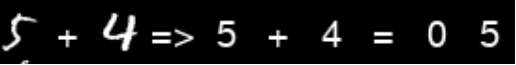
\includegraphics[max width=\textwidth]{tc-fo-example}
	\caption{Example of a TC/FO operation. The operation 5 + 4 is classified correctly, however the output is still false.}
	\label{fig:tc-fo-example}
\end{figure}

This limitation can be due to the fact that the noisy handwritten digits still retain some influence over the network that forces the model to use the noisy inputs for pattern matching instead of the clearer internal representations. Figure \ref{fig:tc-fo-example} shows an example of one of the TC/FO cases trained with 50\% symbols. The handwritten digits are shown along with the result of classification and the result of the operation. The operation is that of 5 + 4. The handwritten digits are classified correctly, however the output of 5 is incorrect. This example shows that the model was still being influenced by the confusing handwritten digits. It might have confused the first operand 5 for the digit 1.

Looking at the results in Table \ref{tab:experiment-3-results-epochs} we see that the more symbols are used the longer it takes for the network to converge onto an optimum decision function. We initially predicted that providing clearer symbols would make the learning process more efficient, but that apparently is not the case. We now understand that without the symbolic information, the gradient descent algorithm will converge to a local minimum early in the training process resulting in the poor classification results and therefore less accurate mathematical operation output. The introduction of more symbols forces the gradient descent algorithm to search longer for an appropriate representation in weight space that is compatible with both the symbol classification and the mathematical operation output.


\section{Explaining the Role of Symbols} \label{sec:empirical-studies-explaining-the-role-of-symbols}

In the previous set of experiments we showed that our theory holds given that the models trained with the aid of symbols outperformed the models that were trained in the absence of symbols. We also showed that there was not much difference in the effectiveness of both the explicit and implicit forms of providing symbols. The next set of experiments investigate the second objective of our research which is to establish the reason why symbols improve learning in artificial neural networks. We start with an experiment that attempts to show that symbols help the artificial learner discover a general solution to the problem, similar to how they are used by humans. Based on the results, we explain the role that symbols play in the learning process.

\subsection{Experiment 4: Recurrent Neural Network's Ability to Discover an Algorithm for Arithmetic Operations} \label{sec:experiment-4}

\subsubsection{Objective}

In Section \ref{sec:theory-approach-methodology-pattern-matching-vs-learning-an-algorithm} we described two possible methods a neural network can learn to perform these arithmetic operations, either by (1) memorizing the input patterns along with the corresponding output, effectively doing pattern matching, or (2) by learning an algorithm that is able to generalize to patterns that the model has not seen before. In the prior experiments, we have shown the former to be true. However, we wish to show that with the aid of appropriate symbols a recurrent neural network is capable of discovering a representation of an algorithm that performs the corresponding mathematical operation.

In this experiment, we attempt to understand whether or not recurrent neural networks are able to accomplish that goal. To verify if that is indeed the case, we train our models on a subset of the combinations of digits. The remaining set of combinations are used to test the trained models. If the models perform well on this unseen set of combinations, this would show that the recurrent neural networks are able to generalize to unseen combinations of digits and is therefore proof that the machine learning system has discovered an algorithm for the arithmetic operations. Otherwise the models trained in the previous experiments are simply doing pattern matching.

\subsubsection{Method}

We develop and train five models for this experiment to perform all four arithmetic operations on the MNIST dataset of handwritten digits. Similar to how the models in Experiment 3 in Section \ref{sec:experiment-3} were trained,  the first model is trained with 0\% symbols, the second with 25\% symbols present, the third with 50\% symbols present, the fourth with 75\% symbols present and finally the fifth with 100\% symbols. All five models have the same architecture that accepts a sequence of three 28x28 images. The first two images are of the handwritten digits representing the operands of the operation. The third image is that of the operator. The models output two one-hot vectors. For the first two time steps the output is the one-hot vector representation of the input digits. On the third step the output is a one-hot vector representation of the result of the operation. Two hidden layers are used each with 512 LSTM units.

The five datasets used in Experiment 3 are also used for this experiment. The difference is that not all combinations of digits are used for training. For each of the five datasets, a subset composed of 80\% of the digit combinations are selected for training for each of the four operators, making sure that each unique digit would be present at least once on either side of the arithmetic operator. We call this the ``seen" dataset since the models are exposed to these combinations during training. The remaining 20\% combinations are the ``unseen" test set that we use to determine if the models are able to generalize to unseen operations and therefore are able to learn an algorithm. The samples in the seen training set are distributed into training, validation and test sets using k-fold cross-validation where k is set to 5. All the samples in the unseen test set are used for testing after the models are trained on the seen dataset. The networks are trained using the Adam optimizer with the mean square error as the loss function and a learning rate of 0.001. Training is performed over 200 epochs in batches of 100 and the model performing best on the validation set is saved and used for testing.

\subsubsection{Results}

\begin{table}[p!]
	\center
	\caption{A comparison of the mean accuracy and standard deviation along with the p-value of a hypothesis t-Test when compared to the 0\% symbols model when tested on the test set of \textbf{seen} combinations.}
	\label{tab:experiment-4-results-table-seen}
	\begin{tabular}{ |c|c|c|c| } 
		\hline
		\% Symbols Present & Accuracy (\%) & Standard Deviation  & p-value\\ 
		0\% & 40.68 & 0.0420 & NA \\  
		25\% & 57.48 & 0.0211 & 0.00383\\  
		50\% & 61.38 & 0.0504 & 0.0 \\  
		75\% & 69.44 & 0.0136 & 0.0\\  
		100\% & 78.23 & 0.0134 & 0.0\\  
		\hline
	\end{tabular}
\end{table}

\begin{table}[p!]
	\center
	\caption{A comparison of the mean accuracy and standard deviation along with the p-value of a hypothesis t-Test when compared to the 0\% symbols model when tested on the test set of \textbf{unseen} combinations.}
	\label{tab:experiment-4-results-table-unseen}
	\begin{tabular}{ |c|c|c|c| } 
		\hline
		\% Symbol Presence & Accuracy (\%) & Standard Deviation  & p-value\\ 
		0\% & 1.00 & 0.0 & NA \\  
		25\% & 3.00 & 0.0240 & 0.374\\  
		50\% & 4.00 & 0.0367 & 0.208 \\  
		75\% & 2.00 & 0.0240 & 0.621\\  
		100\% & 3.00 & 0.0392 & 0.477\\  
		\hline
	\end{tabular}
\end{table}

\begin{figure}[p!]%
	\centering
	\subfloat[Seen Test Combinations]{{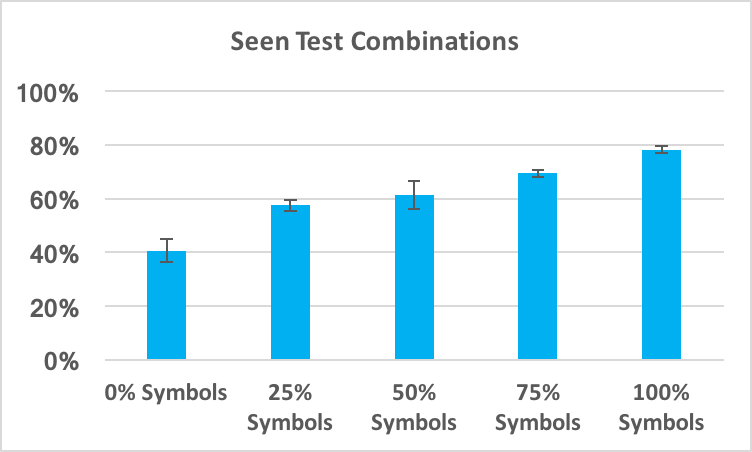
\includegraphics[width=0.5\textwidth]{experiment-4-results-chart-seen}}}%
	\subfloat[Unseen Test Combinations]{{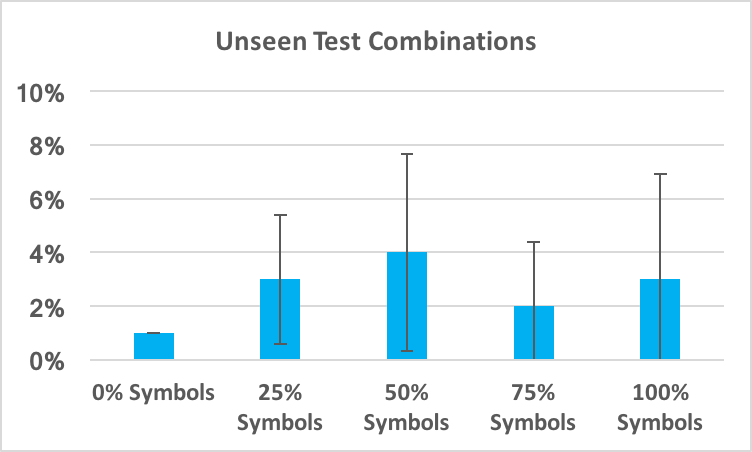
\includegraphics[width=0.5\textwidth]{experiment-4-results-chart-unseen}}}%
	\caption{A comparison of the mean accuracy and 95\% confidence intervals for each of the models when tested on both the \textbf{seen} and \textbf{unseen} test combinations.}
	\label{fig:experiment-4-results-chart}
\end{figure}

Table \ref{tab:experiment-4-results-table-seen} shows the mean accuracy, standard deviation and t-test p-value scores for the test set which uses the same operand combinations that the models were trained on. Table \ref{tab:experiment-4-results-table-unseen} shows these same metrics when the same models are tested on operand combinations they have never seen before. Figure \ref{fig:experiment-4-results-chart} shows graphs of these results along with 95\% confidence intervals.

Table \ref{tab:experiment-4-results-table-seen} shows similar accuracies to those obtained in Experiment 2 with the models trained in the presence of symbols outperforming the ones trained without symbols. However, the models when tested on the unseen dataset show poor performance regardless of whether they are trained with symbols or not.

\subsubsection{Discussion}

It is clear from these results that the current recurrent neural network models are unable to generalize to unseen combinations of operands. They are unable to discover a representation for an algorithm for the arithmetic operations. The models perform well on the previously experienced combinations by developing a sequential mapping function for those seen operand combinations.

In the next section, we describe an experiment that examines our theory in Section \ref{sec:theory-approach-methodology-pattern-matching-vs-learning-an-algorithm} to understand how this pattern matching works and how the presence of symbols makes this process more effective. Later, we present a different approach that uses a modified representation of the symbols as discussed in Section \ref{sec:theory-approach-methodology-temperature-encoding}. Using this new representation, we are able to develop a model that performs well on unseen test sets.

\subsection{Experiment 5: Using Symbols Only to Learn Arithmetic Operations} \label{sec:experiment-5}

\subsubsection{Objective}

We have shown that the presence of symbols improves the accuracy of learning with a limited dataset of noisy examples. In Experiment 3 in Section \ref{sec:experiment-3}, we showed that this was due to the effectiveness of symbols at learning a mapping function. In the previous experiment however, we have failed to show that symbols allow neural networks to go beyond learning mapping functions and actually discover an algorithm to perform the arithmetic operations. In this experiment, we constrain and simplify the problem to make it easier for the models we are developing to reach the desired objective of learning an algorithm. We will train recurrent neural networks to perform addition using the symbolic features alone without introducing the MNIST handwritten digits. The goal here is the same as that of Experiment 4 in Section \ref{sec:experiment-4} where we want to force the network to generalize to unseen combinations of digits.

Besides constraining the input features, we also take a different approach to analyzing the behavior of the trained recurrent neural networks, by visualizing the outputs of the hidden layers of the models using a concept know as activations clustering. With activations clustering, the output value of each unit in the hidden recurrent layers ($h_t$) is mapped to a pixel intensity where an output of -1 would map to 0 and an output of 1 would map to 255. Each unit would be assigned a region on an image and that region would be filled using the pixel intensity assigned when a digit is presented to the trained model on each time step. Figure \ref{fig:activations-cluster-explained} shows an example of an activations cluster. The activations clusters should allow us to confirm that the presence of symbols allows for more consistency in the representation which leads to the improved accuracy. The clusters may also shed some insight into why the networks fail to develop an algorithm.

We will also add an additional time step to the recurrent sequence. Like before, the first time step is the right hand operand, the second time step is the left hand operand, the third time step is the operator which now only outputs the least significant digit of the result. The additional fourth time step is an equals sign which signifies to the model to output the most significant digit of the result. This change was made so that we can determine if there is any relationship between what is being output on the least significant one-hot vector and the most significant one. This also resembles how we as humans do addition. We consume one input digit at a time and we produce one output digit at a time, making note of carry forward digits, if necessary.


\subsubsection{Method}

\begin{figure}
	\centering
	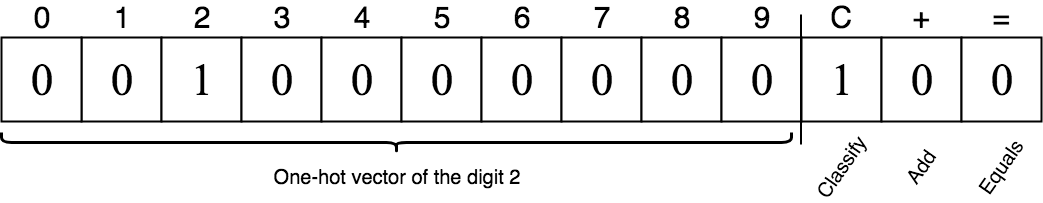
\includegraphics[max width=\textwidth]{experiment-5-input}
	\caption{An example of an input vector for the digit 2 on the first time step. The first ten features are for the one-hot symbol. The 11th (C) feature when set, feature instructs the RNN to output the class at that time step. The 12th (+) feature when set, instructs the network to output the least significant digit of the result. The 13th (=) feature when set, instructs the RNN to output the most significant digit of the result.}
	\label{fig:experiment-5-input}
\end{figure}

The models developed for this experiment accept a sequence of four vectors, each vector is composed of thirteen elements. Figure \ref{fig:experiment-5-input} depicts the structure of the input vectors. The first ten elements represent the one-hot vector. Element 11 is set to one when we want the network to perform classification and output a one-hot vector representing the input operand, zero otherwise. This is always set to one when the operands are presented to the network to signify to the network that an input symbol is being presented on the intermediate time steps. Element 12 is set to one at the third time step. This element indicates that the addition should be performed and that the least significant digit of the output should be produced. The element is set to zero otherwise. Finally, element 13 is set to one on the fourth time step when the most significant digit of the result of the addition is presented on the output.

\begin{figure}
	\centering
	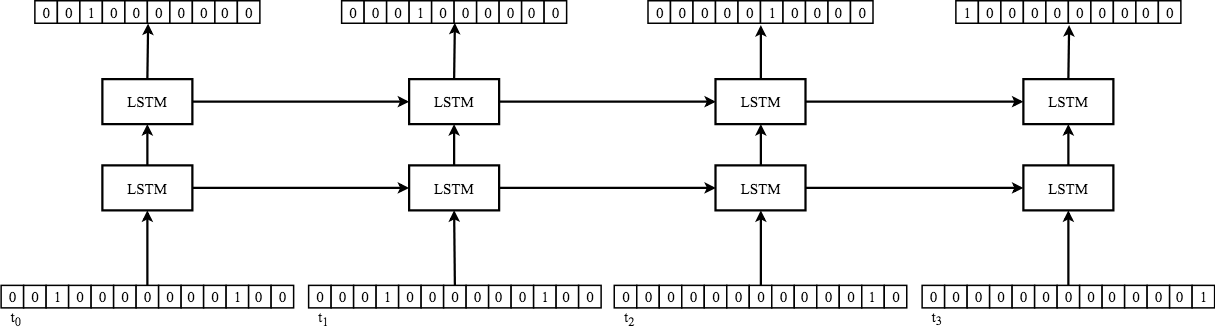
\includegraphics[max width=\textwidth]{experiment-6-architecture}
	\caption{The constrained symbol only architecture learning to perform 2 + 3.}
	\label{fig:experiment-6-architecture}
\end{figure}

The output layer of the models consists of 10 elements representing a one-hot vector output. When the first operand is presented on the input layer, the network outputs the same digit on the output layer. The same goes for the second operand on the second time step. When an input that has the 12th element set to one is presented on the third time step, the network outputs the least significant digit of the result of adding the operands together. Finally, on the fourth time step when an input having the 13th element set to one is presented to the model, the model outputs the most significant digit of the addition. Figure \ref{fig:experiment-6-architecture} depicts how the input and output layers interact on each time step.

A total of four recurrent neural network architectures were developed using the same input and output layer structures presented above. The models vary in the number and size of the recurrent hidden layers.  The following lists the composition of the hidden layers for each of the four models developed:
\begin{itemize}
	\item \textbf{Model A}: One hidden layer with 10 LSTM units each.
	\item \textbf{Model B}: Two hidden layers with 10 LSTM units each.
	\item \textbf{Model C}: Three hidden layers with 10 LSTM units each.
	\item \textbf{Model D}: Two hidden layers with 20 LSTM units each.
\end{itemize}

The dataset is composed by forming all possible 100 combinations of operands. A subset of 80 combinations are selected for training from that dataset, making sure that each unique digit would be present at least once on either side of the addition operator. That same training set is also used for validation and as the test set of seen combinations. The remaining 20 combinations are used as the unseen combinations test set. Each model is trained and tested five times and the mean accuracy of each model is recorded when applying both the seen test set and the unseen test set on the trained model. Training is performed over 5000 epochs in batches of 10 using the Adam optimizer algorithm and the mean square error loss function with a learning rate of 0.001.

\subsubsection{Results}

\begin{figure}
	\centering
	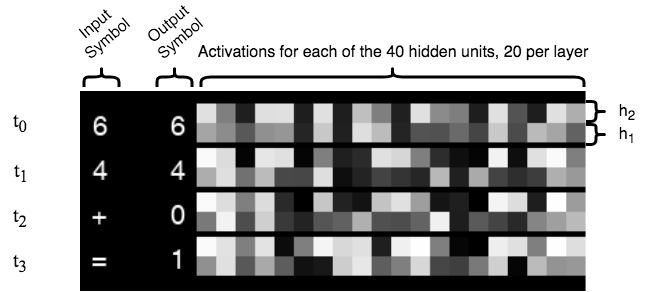
\includegraphics[max width=\textwidth]{activations-cluster-explained}
	\caption{An activations cluster generated when presenting the one-hot symbols of the operation 6 + 4 to the trained Model D. The symbols are displayed in this image as digits for clarity.}
	\label{fig:activations-cluster-explained}
\end{figure}

Table \ref{tab:experiment-6-results-table} shows the mean accuracies for each of the architectures developed. The table shows these values for both the full training set and the unseen test set. Figures \ref{fig:activations-cluster-explained} and \ref{fig:activations-cluster-carry} show some of the activations clusters that are produced when applying the seen dataset to Model D (the best performing model).

Figure \ref{fig:activations-cluster-explained} shows the result of rendering the activations cluster when applying the operand sequence of 6 + 4 to the trained Model D. The figure shows four rows of items, each row represents a single time step. For each time step, the figure depicts the input to the network, the output the network produces and the activations on the hidden units. The inputs and outputs are rendered in the figure as digits for clarity. Forty activations are shown for each time step, one for each hidden unit. The activations are split into two rows, each row holds the activations for one of the two hidden layers.

\begin{table}[h]
	\center
	\caption{A comparison of the mean accuracy of each of the four models developed when tested on the test set of \textbf{seen} combinations as well as the test set of \textbf{unseen} combinations.}
	\label{tab:experiment-6-results-table}
	\begin{tabular}{ |c|c|c| } 
		\hline
		Model & Accuracy - Seen (\%) & Accuracy - Unseen (\%)\\ 
		Model A & 75.0 & 5.0\\  
		Model B & 75.0 & 5.0\\  
		Model C & 75.0 & 5.0\\  
		Model D & 100.0 & 5.0\\
		\hline
	\end{tabular}
\end{table}

\subsubsection{Discussion}

It is clear from the results that even when constraining the model to only use one-hot symbols as inputs, the recurrent networks fail to generalize to the unseen dataset, even though they perform very well on the seen dataset. This shows that even when using clear one-hot symbols the neural network is still not able to discover a set of weights that can represent an algorithm that performs the addition operation.

\begin{figure}
	\centering
	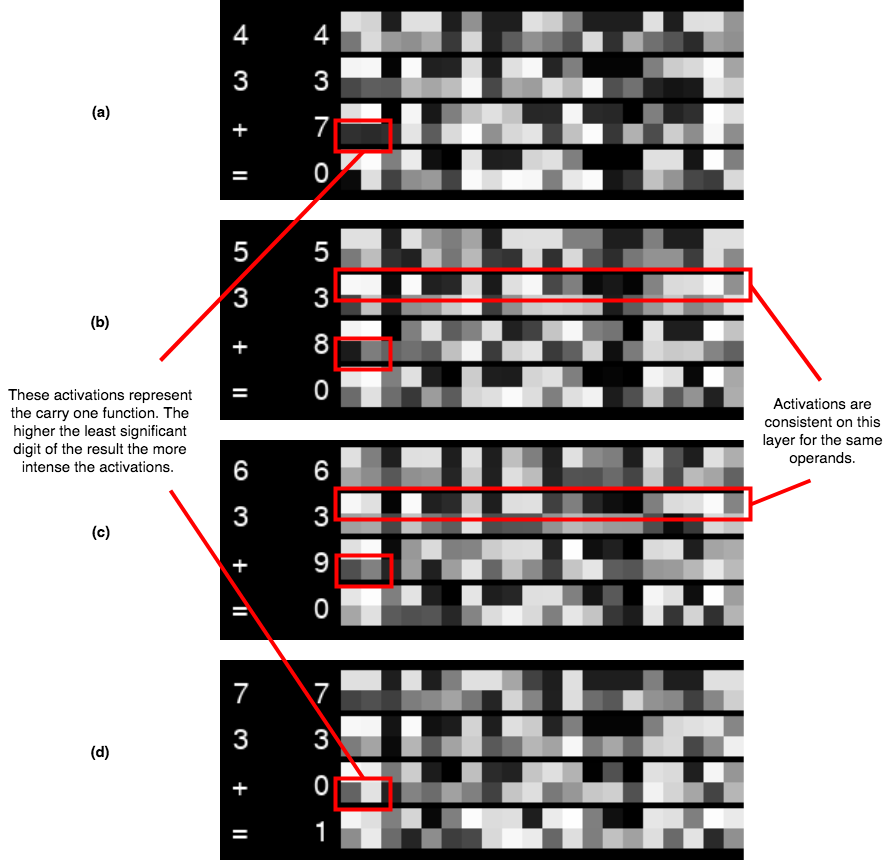
\includegraphics[max width=\textwidth]{activations-cluster-carry-annotated}
	\caption{A series of activations from Model D showing how the intensity in the bottom left region of the third time step changes when the output transitions from 7 through 8 and 9 to 10.}%
	\label{fig:activations-cluster-carry}%
\end{figure}

When analyzing the sequence of activations clusters in Figure \ref{fig:activations-cluster-carry}, we notice that the activations on the top layer ($h_2$) on any of the first two time steps are always consistent when the same operands are presented as exhibited by the digit 3 on the second time step of Figures \ref{fig:activations-cluster-carry} (a) to \ref{fig:activations-cluster-carry} (d). Also, the least and most significant digit outputs always have consistent activations on the top layer for the same results (see the fourth time step in Figures \ref{fig:activations-cluster-carry} (a), \ref{fig:activations-cluster-carry} (b) and \ref{fig:activations-cluster-carry} (c) and the third time step in Figure \ref{fig:activations-cluster-carry} (d)). By ``consistent" we mean that the same hidden units are producing the same intensities. These observations are in-line with the findings of Experiment 3 in Section \ref{sec:experiment-3} which shows that when successfully classifying the input digits, the recurrent neural networks discover a consistent internal representation that facilitates the execution of the arithmetic operations.

Another interesting pattern can be observed when analyzing the transition from the least significant digit time step to the most significant digit time step (see Figure \ref{fig:activations-cluster-carry}). The two most left-hand activations on the lower layer of the third (least significant digit) time step tend to be dark (indicating lower activations) when the least significant digit of the result is closer to zero than nine. The higher that digit the lighter the activations become. The variation in activations indicates that there is a signal being carried over from the least significant digit time step to the most significant digit time step. That signal forces the most significant output to flip from a zero to a one. When comparing this behavior with how we as humans perform addition, this process resembles the carry-one approach when writing out arithmetic problems with pen and paper. This shows that though for the most part the networks are still learning a mapping function, there are still some elements of an algorithm being developed within the network.

When further analyzing how humans learn to perform addition, we tend to convert the numbers into concepts that can be counted. More specifically with children, we represent numbers as collections of objects. So, 5 + 3 for example will be translated to a child as counting five ``apples" and counting another three ``apples" on top of the initial five. The symbols are able to represent quantity and ordinal relationships. One-hot vectors on the other hand don't capture these concepts; they are able to represent classes of digits which is why they assist in the development of good classifiers, but fail to develop models that can generally perform arithmetic. In the next set of experiments we use a different encoding for our symbols that better captures the ordinal nature of the digits.

\section{Temperature Encoding Experiments} \label{sec:empirical-studies-temperature-encoding-experiments}

So far we were able to show that symbols improve the effectiveness of the learning process when training neural networks on limited datasets. We have however failed to show that they can generalize to digit combinations that they have not seen before. In Section \ref{sec:theory-approach-methodology-temperature-encoding} we described an alternative representation for our symbols, namely the temperature encoded symbols. We explained our expectation that temperature encodings will improve the ability of the networks to generalize to unseen combinations since they are able to encapsulate three characteristics that are important in developing an algorithm that performs arithmetic. Specifically, these characteristics are, (1) the ability of the symbols to represent the ordinal relationship between digits, (2) the ability to represent the quantity of the digits and (3) the ability to capture the function of the operator. The prior experiment showed that one-hot vectors are capable of capturing the function of the operator, as shown by the ability of the models to internally represent the carry forward behavior of addition. They however fail in providing the other two properties. This final set of experiments investigates the ability of temperature encoded symbols to capture all three characteristics and presents a solution to our problem. 

\subsection{Experiment 6: Temperature Encoding} \label{sec:experiment-6}

\subsubsection{Objective}

When a symbol is represented as a temperature encoded vector, the symbol is represented as an array where a number of consecutive elements equal to the value of the digit being represented are set to one, the rest are set to zero. Figure \ref{fig:temperature-encoding} shows a depiction of a temperature encoded symbol of the number 5. We believe that symbols encoded using this representation can capture the quantitative and ordinal meaning of the digits and would therefore help the recurrent neural network learn an algorithm for arithmetic operations as opposed to simply learning a classifier or mapping function.

The goal of this experiment is to determine empirically whether or not models trained using the temperature encoded symbols have the ability to discover a decision function that can represent the algorithm that performs addition. We constrain the experiment to only use symbols as in Experiment 5. The models accept a sequence of operands encoded in the temperature encoding and outputs values encoded in the temperature encoding as well. The performance of the trained model is tested against both the training set as well as an unseen test set to determine if the model can generalize to unseen combinations of operands. 

\subsubsection{Method}

\begin{figure}
	\centering
	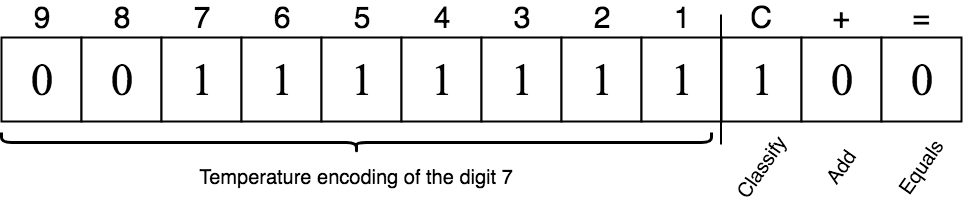
\includegraphics[max width=\textwidth]{experiment-6-input}
	\caption{An example of an input vector for the digit 7 on the first time step. The first nine features are for the temperature encoded symbol. The 10th (C) feature when set, instructs the RNN to output the class at that time step. The 11th (+) feature when set, instructs the network to output the least significant digit of the result. The 12th (=) feature when set, instructs the RNN to output the most significant digit of the result.}
	\label{fig:experiment-6-input}
\end{figure}

Three models are developed that learn to perform addition on temperature encoded symbols. Figure \ref{fig:sequential-model-temperature-symbols} shows an example of a recurrent neural network using temperature encoding to learn to do addition. The models accept a sequence of four vectors 12 elements each. Figure \ref{fig:experiment-6-input} depicts an example input. The first nine elements hold an operand represented as a symbol encoded using a temperature encoding. The 10th element indicates to the network to classify the input, meaning that if it is set to one, the model should output the same input digit using the same temperature encoding. The 11th element indicates the addition operator and the model should output the least significant digit of the result of the addition. Finally, the 12th element represents the equals sign, indicating to the model to output the most significant digit of the result. The output of each of the networks is a nine-element vector that represents the temperature encoding of the output. The following are the various architectures that were tried:
\begin{itemize}
	\item \textbf{Model A}: Two hidden layers, 20 units each.
	\item \textbf{Model B}: Two hidden layers, 10 units each.
	\item \textbf{Model C}: Two hidden layers, 5 units each.
\end{itemize}

\begin{figure}
	\centering
	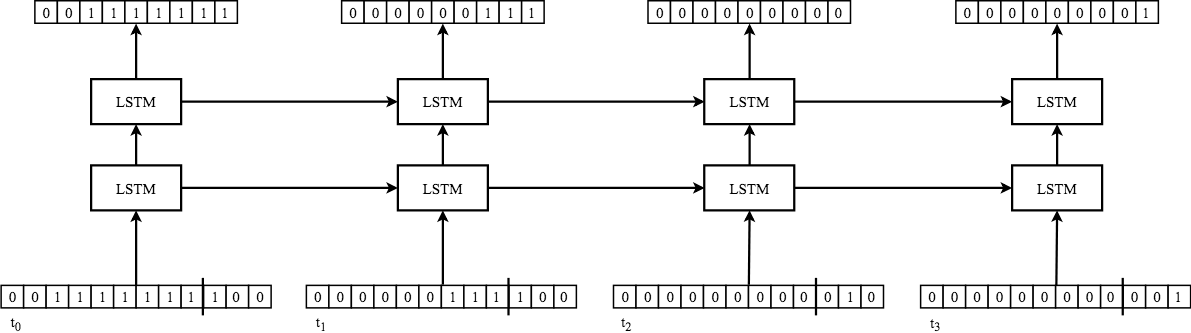
\includegraphics[max width=\textwidth]{sequential-model-temperature-symbols}
	\caption{A sequential model constrained to use symbols only. However, the symbols are encoded using temperature encoding. In this case the model is learning to perform 7 + 3. The output on the third time step (least significant time step) is all zeros to encode 0.}
	\label{fig:sequential-model-temperature-symbols}
\end{figure}

A similar dataset like the one used in Experiment 5 is used for this experiment. A subset of 80 combinations are selected for training from the 100 combinations of operands, making sure that each unique digit would be present at least once on either side of the addition operator. That same training set is also used for validation and as the test set of seen combinations. The remaining 20 combinations are used as the unseen combinations test set. Each model is trained and tested five times and the mean accuracy of each model is recorded when applying both the seen test set and the unseen test set on the trained model. Training is performed over 5000 epochs in batches of 10 using the Adam optimizer algorithm and the mean square error loss function with a learning rate of 0.001. 

\subsubsection{Results}

\begin{table}
	\center
	\caption{A comparison of the mean accuracy of each of the models trained using the temperature encoding when tested on the test set of \textbf{seen} combinations as well as the test set of \textbf{unseen} combinations.}
	\label{tab:experiment-7-results-table}
	\begin{tabular}{ |c|c|c| } 
		\hline
		Model & Accuracy - Seen (\%) & Accuracy - Unseen (\%)\\ 
		Model A & 100.0 & 90.0\\  
		Model B & 100.0 & 93.0\\  
		Model C & 100.0 & 86.0\\  
		\hline
	\end{tabular}
\end{table}

Table \ref{tab:experiment-7-results-table} shows the results obtained for each of the architectures trained. The table presents the mean accuracies of each architecture when tested on both the dataset of seen combinations and the dataset of unseen combinations. 

\subsubsection{Discussion}

\begin{figure}
	\centering
	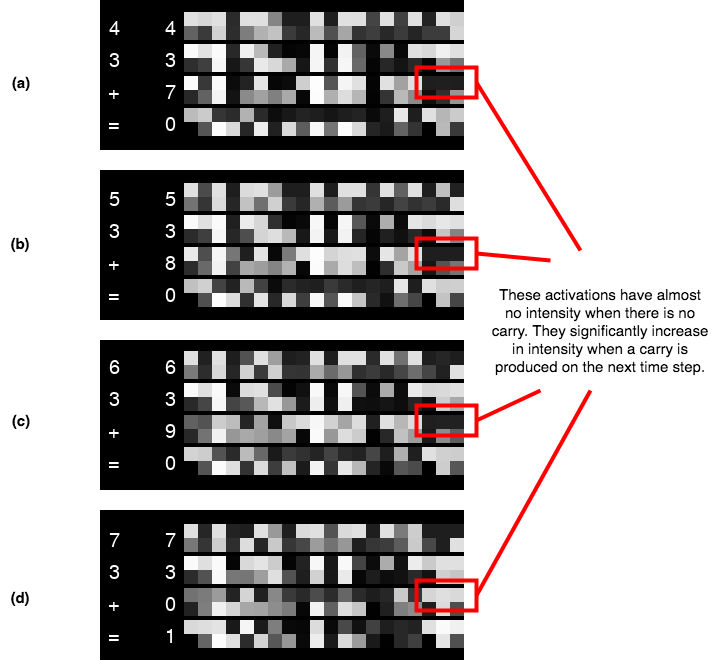
\includegraphics[max width=\textwidth]{activations-cluster-carry-temperature}
	\caption{A series of activations produced when applying examples from the unseen test set to Model A, trained using temperature encoded symbols. The activations show how the intensity in the top right region of the third time step indicates if a carry should be generated.}%
	\label{fig:activations-cluster-carry-temperature}%
\end{figure}

We can see from the results in Table \ref{tab:experiment-7-results-table} that the models perform perfectly on the training combinations and are also relatively successful at generalizing to the unseen combinations. This shows that the temperature encoded symbols that take into account the ordinal nature of the digits allow the recurrent neural networks to capture an algorithm that performs addition.

\begin{figure}%
	\centering
	\subfloat[Activations for 4 + 3]{{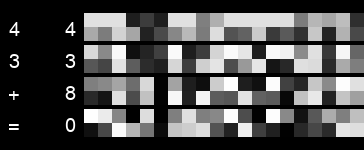
\includegraphics[width=0.5\textwidth]{activations-cluster-no-carry-4-3} }}%
	\subfloat[Activations for 5 + 3]{{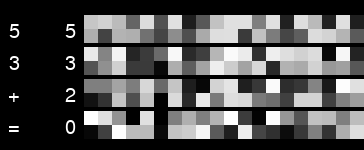
\includegraphics[width=0.5\textwidth]{activations-cluster-no-carry-5-3} }}%
	
	\subfloat[Activations for 6 + 3]{{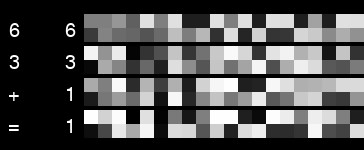
\includegraphics[width=0.5\textwidth]{activations-cluster-no-carry-6-3} }}%
	\subfloat[Activations for 7 + 3]{{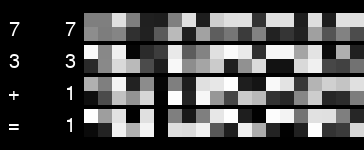
\includegraphics[width=0.5\textwidth]{activations-cluster-no-carry-7-3} }}%
	\caption{A series of activations produced when applying examples from the unseen test set to Model D of Experiment 5, trained using one-hot vector symbols. No discernible patterns are visible.}%
	\label{fig:activations-cluster-no-carry}%
\end{figure}

To further verify this conclusion, we generated activations clusters for a series of combinations from the unseen test set using Model A. Figure \ref{fig:activations-cluster-carry-temperature} shows the activations produced. In addition, Model D from the previous experiment (Experiment 5 in Section \ref{sec:experiment-5}) was retrained making sure that the same combinations shown in Figure \ref{fig:activations-cluster-carry-temperature} are part of the unseen test set. The activations for that model are shown in Figure \ref{fig:activations-cluster-no-carry}. The activations generated by the model trained using the temperature encoded symbols exhibit consistency among the same operands. Also, the region indicated at the top right end of the third time step shows a clearer carry forward signal than the one seen in Figure \ref{fig:activations-cluster-carry-temperature}. When we contrast these activations with the ones shown in Figure \ref{fig:activations-cluster-no-carry} we see that the model trained with one-hot vector symbols do not depict these clear patterns when applied to the unseen test set.

Experiments 5 and 6 show that symbols improve the accuracy of neural networks by aiding the learning algorithm in discovering a representation that capture some aspects of the algorithm that performs the operation. Temperature encoded symbols allow the models to capture more aspects. Specifically, the quantity and ordinal relationship of the operands. This results in better generalization. In the next and final experiment, we replicate Experiment 4 but this time, instead of using the one-hot vectors we use temperature encoded symbols.

\subsection{Experiment 7: Noisy Handwritten Digits with Temperature Encoded Symbols} \label{sec:experiment-7}

\subsubsection{Objective}

In Section \ref{sec:theory-approach-methodology-temperature-encoding} we explained our observation of how humans learn to perform arithmetic. We explained how children in particular learn to represent digits by mapping between the image of a digit and the image of familiar objects. These familiar objects (like apples for example) behave as symbols that convey both quantity and ordinal relationships. The human learner can then act on these symbols to produce a more accurate result. This process allows the human learner to generalize the solution to combinations of digits that they have not experienced before.

We believe a neural network model can be constructed that learns in a similar way. The network is provided a sequence of handwritten digits and an operator symbol. It is trained to develop an internal representation that can map between the image of the digit and a symbol that captures both the quantity and ordinal relationships represented by the digit (the temperature encoded symbol). The model is also trained to perform the arithmetic operation on the two digits. With deep recurrent neural networks, these two related tasks can be combined into one model that can learn to perform both with high accuracy.

The purpose of this experiment is to show that it is indeed possible to build such a model and that the use of symbols represented as temperature encodings can improve the accuracy of training on a restricted dataset as well as force the learning algorithm to discover a representation that can generalize to unseen combinations of digits. We also investigate how varying the amount of symbols present affects the accuracy of the model on the unseen test data.

\subsubsection{Method}

Five recurrent neural network models are developed for this experiment each having the same architecture. Figure \ref{fig:sequential-model-noisy-temperature} shows a diagram of the architecture used. The models accept a sequence of four 28x28 images. The first two images are of the MNIST handwritten digit operands, the third image is the operator (plus, minus, times and divide) consistently rendered in a standard font, and finally the fourth image is an equals sign. The model is trained so that when it sees the operands on each of the first two time steps, it outputs a temperature encoded symbol that represents the digit in the image. When the model is presented with the operator on the input, it performs the operation on the operands and then outputs a temperature encoded symbol that represents the least significant digit of the result. Finally, when the equals sign is presented, the model outputs a temperature encoded symbol representing the most significant digit of the result.

The neural network architecture used is composed of an input layer of 784 units for the 28x28 pixel images. Two hidden layers are used each consisting of 512 LSTM units. The output layer is a vector of nine elements to represent the temperature encoded results. The networks are trained using the Adam optimizer with the mean square error as the loss function and a learning rate of 0.001. Training is performed over 200 epochs in batches of 100 and the model performing best on the validation set is saved.

\begin{figure}
	\centering
	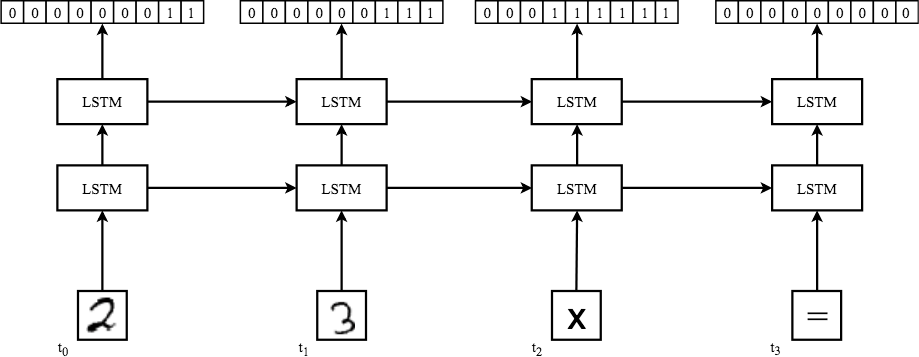
\includegraphics[max width=\textwidth]{sequential-model-noisy-temperature}
	\caption{A sequential model learning to perform arithmetic on images of handwritten digits in the presence of symbols. The symbols are provided on the outputs of the first two intermediate steps using temperature encoding. Here the model is performing multiplication on the combination: 2 x 3.}
	\label{fig:sequential-model-noisy-temperature}
\end{figure}

The same dataset used in Experiment 4 in Section \ref{sec:experiment-4} is also used for this experiment with the exception of replacing one-hot vector symbols with temperature encoded symbols. To recap, for each operator, the combinations of digits are split into a set of seen combinations that includes, 80\% of the combinations of digits. For each of the seen combinations, eight MNIST samples are selected. Four of these samples are used for training, two for validation and the remaining two for testing. The remaining 20\% of the combinations are reserved as the set of unseen combinations that are used to verify that the models have learned an algorithm of the operations. The dataset of seen combinations is replicated five times, each replica includes a different percentage of symbols present. The symbol spreads used are 0\%, 25\%, 50\%, 75\% and 100\%. The symbols were presented as output labels to the first two time steps. The model is trained to classify the handwritten digit with the aid of the symbol provided. When symbols are not provided, a vector composed of 0.5 dummy values is used instead. Each model is trained five times using 5-fold cross-validation.

\subsubsection{Results}

\begin{table}[p]
	\center
	\caption{A comparison of the mean accuracy and standard deviation along with the p-value of a hypothesis t-Test when compared to the 0\% symbols model when tested on the test set of \textbf{seen} combinations.}
	\label{tab:experiment-8-results-table-seen}
	\begin{tabular}{ |c|c|c|c| } 
		\hline
		\% Symbols Present & Accuracy (\%) & Standard Deviation  & p-value\\ 
		0\% & 41.55 & 0.0302 & NA \\  
		25\% & 51.30 & 0.0457 & 0.02311\\  
		50\% & 60.65 & 0.0379 & 0.00049 \\  
		75\% & 75.84 & 0.0587 & 0.00063\\  
		100\% & 84.26 & 0.0582 & 0.00018\\  
		\hline
	\end{tabular}
\end{table}

\begin{table}[p]
	\center
	\caption{A comparison of the mean accuracy and standard deviation along with the p-value of a hypothesis t-Test when compared to the 0\% symbols model when tested on the test set of \textbf{unseen} combinations.}
	\label{tab:experiment-8-results-table-unseen}
	\begin{tabular}{ |c|c|c|c| } 
		\hline
		\% Symbols Present & Accuracy (\%) & Standard Deviation  & p-value\\ 
		0\% & 4.62 & 0.0133 & NA \\  
		25\% & 25.53 & 0.0900 & 0.16889\\  
		50\% & 45.90 & 0.0319 & 0.00199 \\  
		75\% & 54.63 & 0.0324 & 0.0\\  
		100\% & 69.58 & 0.0694 & 0.00088\\  
		\hline
	\end{tabular}
\end{table}

\begin{figure}[p]
	\centering
	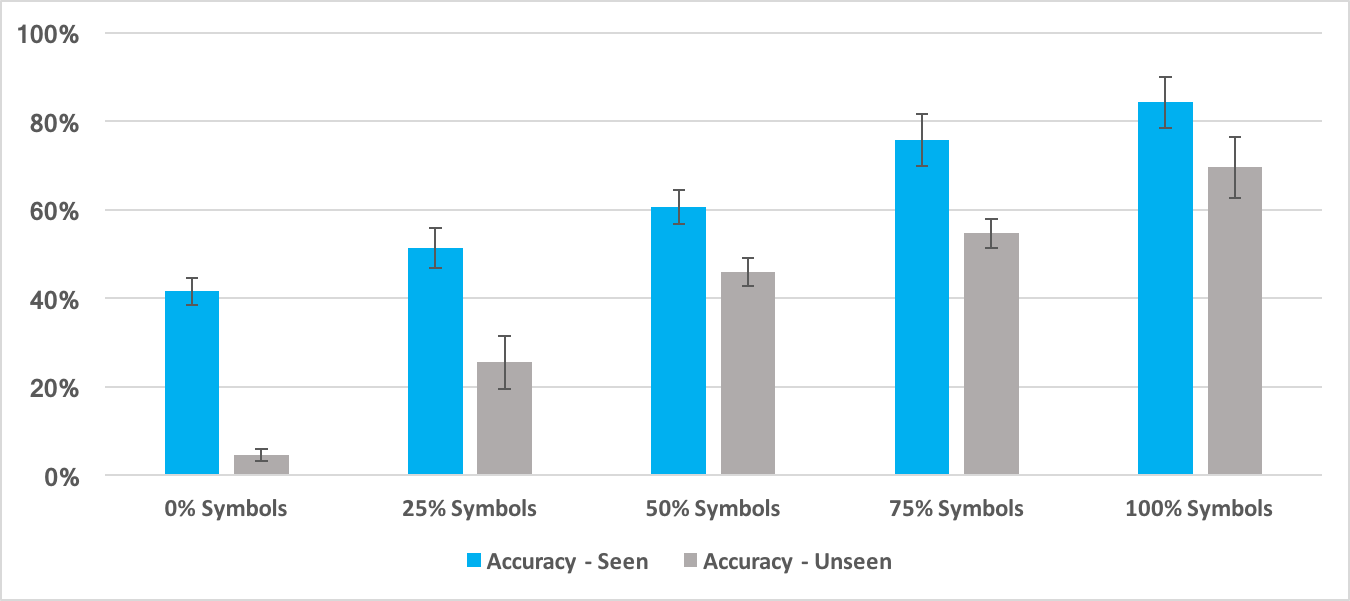
\includegraphics[max width=\textwidth]{experiment-8-results-chart-2}
	\caption{A comparison of the mean accuracy and 95\% confidence intervals for each of the models trained with 0\% to 100\% temperature encoded symbol presence when tested on both the test set of \textbf{seen} and \textbf{unseen} combinations.}
	\label{fig:experiment-8-results-chart}
\end{figure}

Table \ref{tab:experiment-8-results-table-seen} shows the results of testing the models on the test set of seen combinations. Similarly, Table \ref{tab:experiment-8-results-table-unseen} shows the results of testing the model on the test set of unseen combinations. The tables present the mean accuracy, standard deviation and the p-test score for each of the models developed. Figure \ref{fig:experiment-8-results-chart} depicts the mean accuracies along with the 95\% confidence intervals for all five models trained on both the seen and unseen test sets.

\subsubsection{Discussion}

The results show that increasing the number of symbols available per combination during training, improves the accuracy of the recurrent network when tested on combinations the model has seen during training. This result is comparable to Experiment 4 where we had a similar architecture and approach. However, we used a different representation for the symbols, namely temperature encoded vectors. More importantly the results show the accuracy on unseen combinations increases as more symbols are used during training. These results confirm the findings we've observed in several of our previous experiments and also supports our hypothesis that artificial neural networks similar to human learners can benefit from the presence of clear and concise symbols when training using limited datasets.

The results in this experiment show that the way the symbols are represented can have significant effect on the learning ability of the models. The one-hot vector representation was effective for learning a simple mapping function when all combinations of inputs were provided during training. However, it failed to capture the ordinal nature of the digits and therefore they were not able to discover a representation for an algorithm that can perform the arithmetic operations. By using temperature encoded symbols for the digits, the models are able to represent the arithmetic algorithm and generalize to unseen combinations of digits.

\section{Summary} \label{sec:theory-summary}

This chapter presented our basic hypothesis. The theory states that individual human learners struggle to learn new concepts through experimentation alone when the number of examples provided to them is limited. However, through interaction with other learners, common symbols for noisy concepts are shared that allows the learner to overcome the challenges in developing accurate models. We hypothesize that the introduction of such a symbolic channel to an artificial neural network model can also help the model achieve higher levels of accuracy when training with an impoverished dataset.

We also proposed a problem domain to validate this hypothesis, namely to teach artificial neural network models to perform arithmetic on images of handwritten digits. We first explained that the process of learning arithmetic operations can be modeled using sequential neural network architectures. We then presented two methods of supplying symbolic information to these models. Next, two theories were discussed on the role the symbols play in guiding the learning system towards discovering an optimum solution to the problem. Finally, we introduced a new form of symbolic representation, that of temperature encoding, that we believe will capture all aspects of learning to perform arithmetic and will therefore produce the best results. 